\section{Definicje}

\begin{frame}{Uczenie poprzez wzmocnienie}
  \begin{columns}[T,onlytextwidth]
    \begin{column}{0.53\textwidth}
      \begin{itemize}
        \item \textbf{Decydent (agent)} obserwuje stan $s \in S$ i wybiera akcję $a \in A$, aby maksymalizować przyszłe nagrody.
        \item \textbf{Środowisko} opisane jest przez dynamikę $q(s' \mid s,a)$ i funkcję nagrody $r(s,a)$, które określają konsekwencje działań.
        \item \textbf{Polityka} $\phi$ to reguła decyzyjna mapująca stany (lub historie) na rozkłady akcji.
        \item Klasyczny cykl RL: obserwacja $\rightarrow$ decyzja $\rightarrow$ nagroda $\rightarrow$ nowy stan.
      \end{itemize}
    \end{column}
    \begin{column}{0.42\textwidth}
      \centering
      % \includegraphics[width=0.9\linewidth]{../../data/plots/rl_scheme.png}
      % Schemat pętli interakcji agent--środowisko.
      \textit{[Diagram schematu RL]}
    \end{column}
  \end{columns}
\end{frame}

\begin{frame}{Quasi-hiperboliczne uczenie poprzez wzmocnienie}
  \begin{columns}[T,onlytextwidth]
    \begin{column}{0.55\textwidth}
      \begin{itemize}
        \item Wersja quasi-hiperboliczna wzbogaca RL o uprzedzenie teraźniejszości: wagi dyskontowe $d(0)=1$, $d(t)=\alpha\,\beta^{t}$ dla $t \ge 1$.
        \item Parametr $\alpha>0$ zwiększa wartość nagród natychmiastowych, a $\beta \in [0,1)$ zachowuje zależność wykładniczą w przyszłości.
        \item Optymalizacja polityki wymaga pogodzenia krótkoterminowych impulsów z celami długoterminowymi.
        \item Taki model lepiej odzwierciedla decyzje ludzi, którzy preferują wcześniejsze nagrody.
      \end{itemize}
    \end{column}
    \begin{column}{0.4\textwidth}
      \centering
      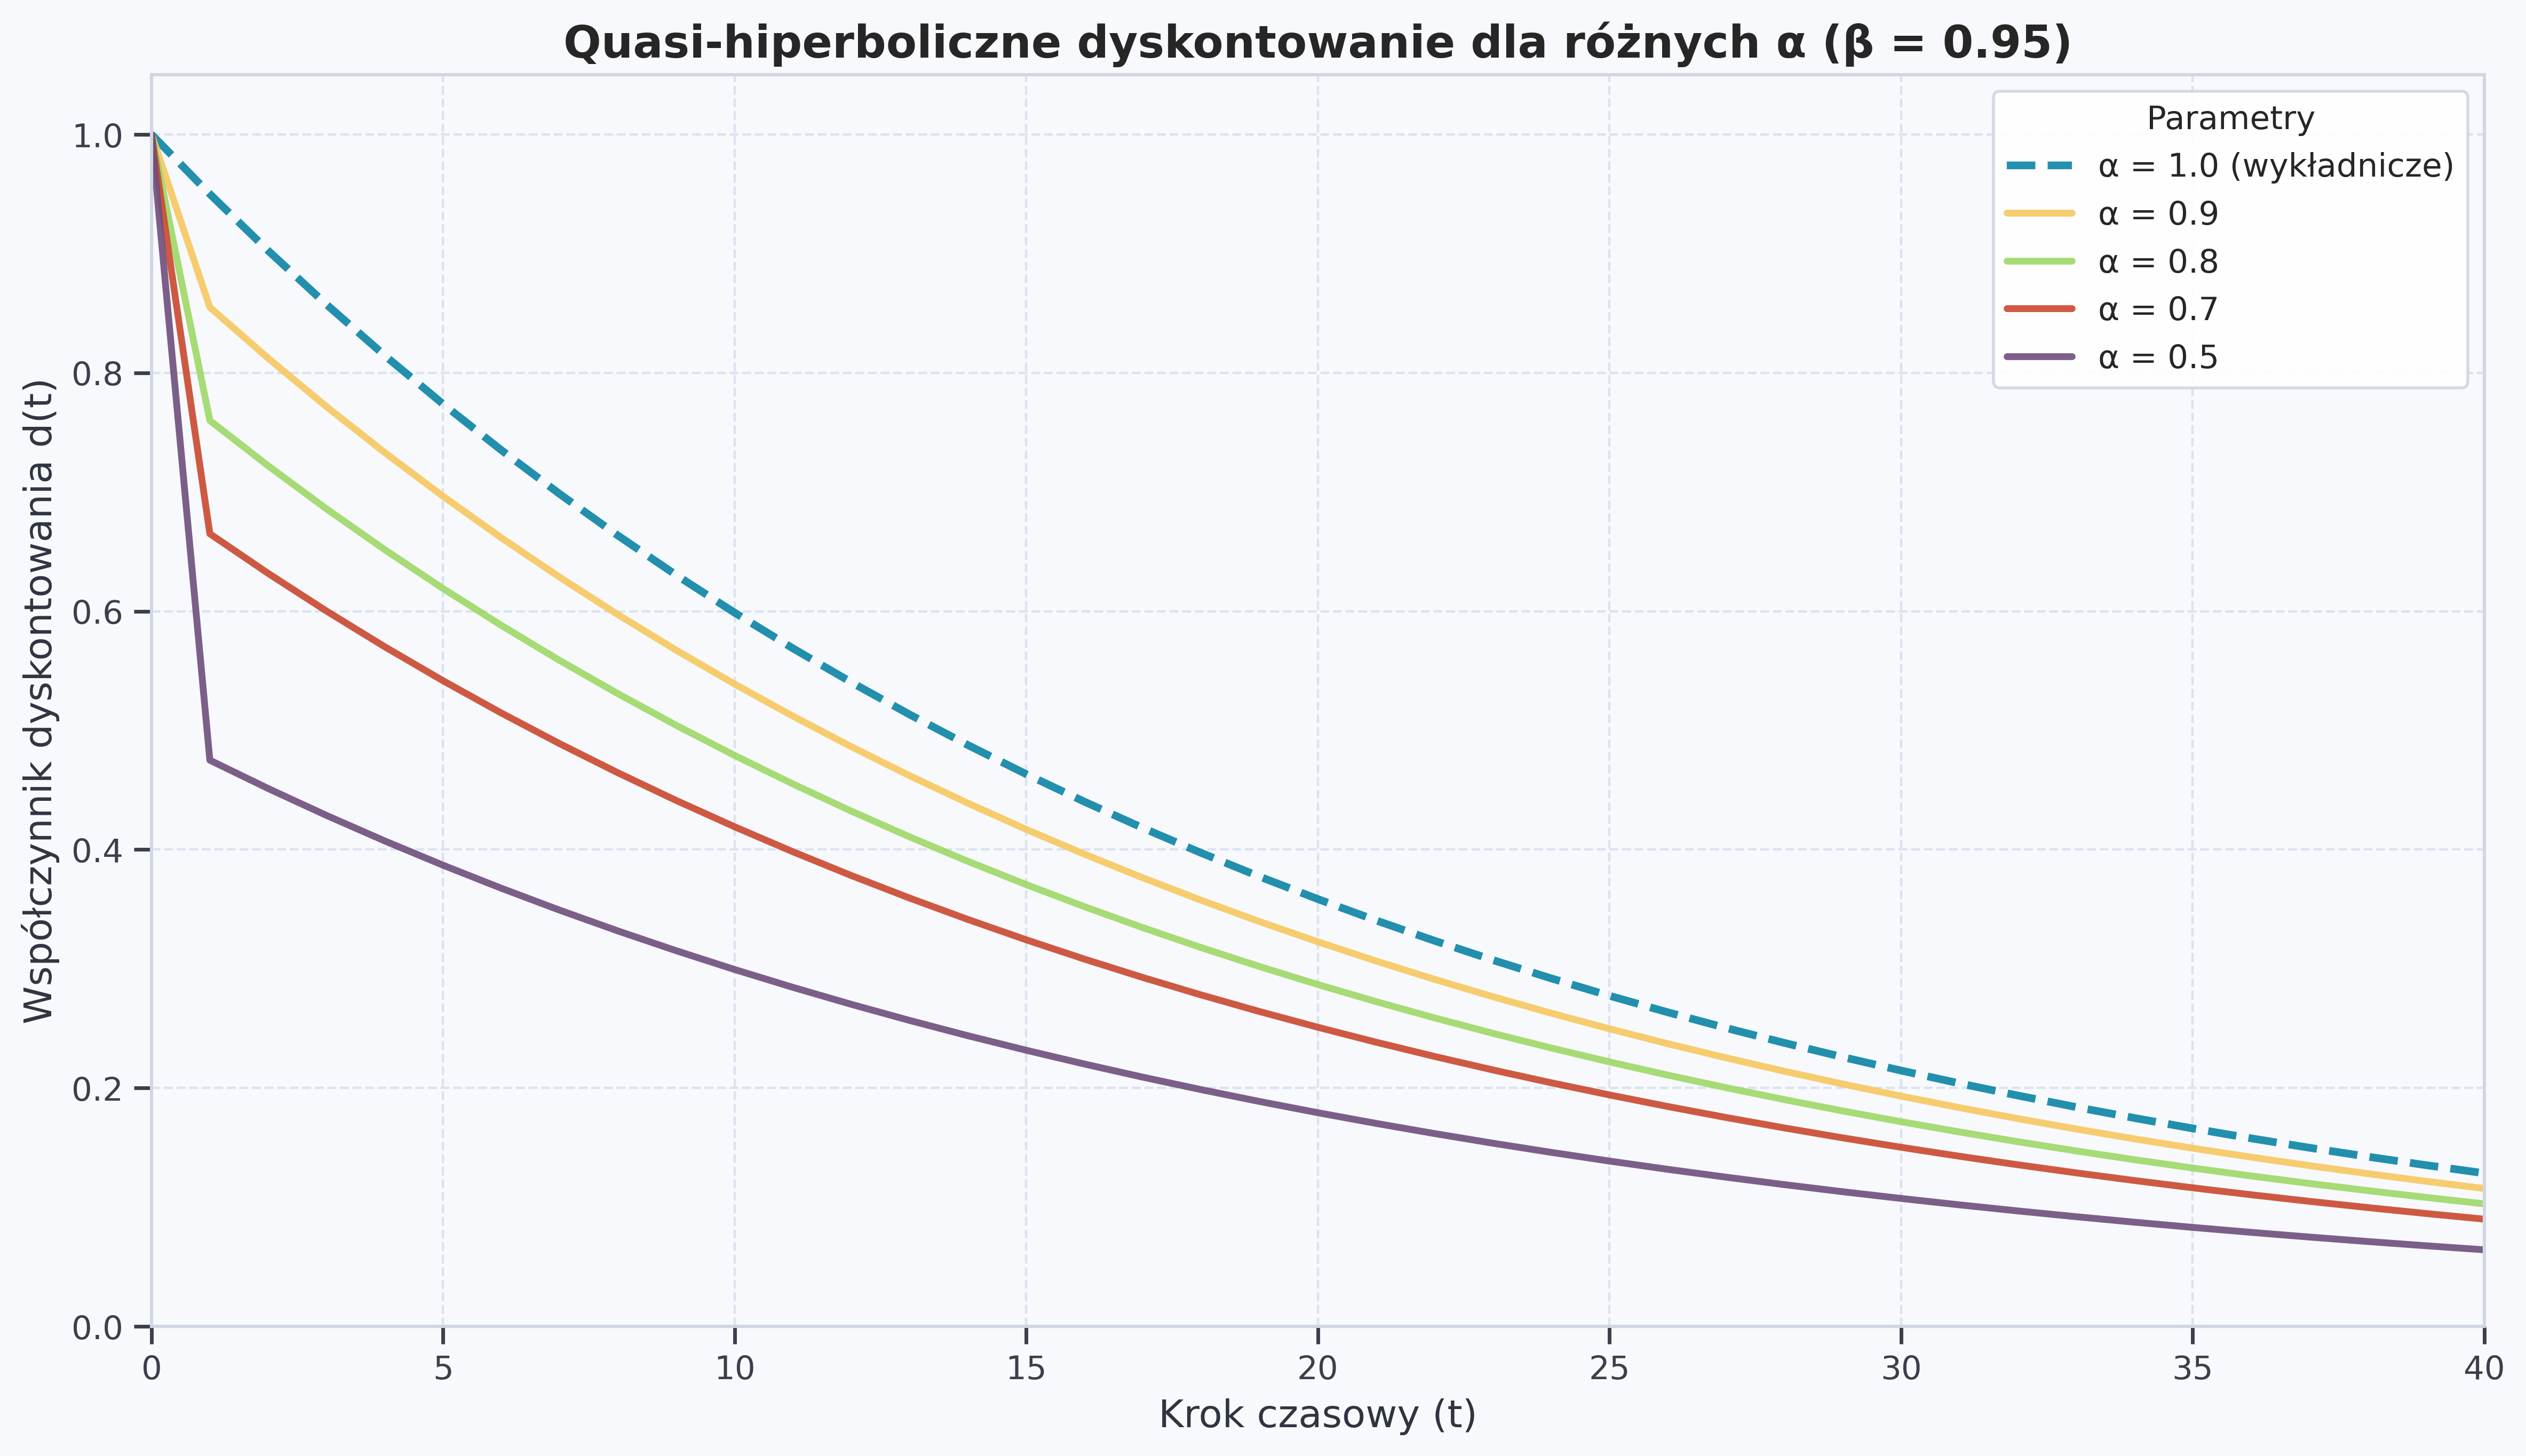
\includegraphics[width=\linewidth]{../../plots/qh_discounting_comparison.png}
      \vspace{0.4em}
      \small Porównanie wag dyskontowych: wykładniczych vs. quasi-hiperbolicznych.
    \end{column}
  \end{columns}
\end{frame}
